\chapter{Diseño del sistema}

En este capítulo se mostrará el desarrollo general del sistema, comenzando por una visión superficial del sistema hasta obtener la versión final del sistema. En capítulos posteriores se mostrará el proceso de diseño e implementación de cada parte del mismo.

\section{Descripción general del sistema}

El requisito fundamental de este trabajo fue poder controlar el sistema de entrada y salida de vehículos de al menos un recinto. Por lo tanto primero se explicará el caso particular de cómo funciona el sistema para el caso de un solo lugar. Adicionalmente existen otros requisitos preestablecidos, como:

\begin{itemize}
    \item Medir el tiempo del vehículo dentro del establecimiento.
    \item Que la entrada y salida sea automática basada en la patente.
\end{itemize}

\begin{figure}[bth]
    \centering
    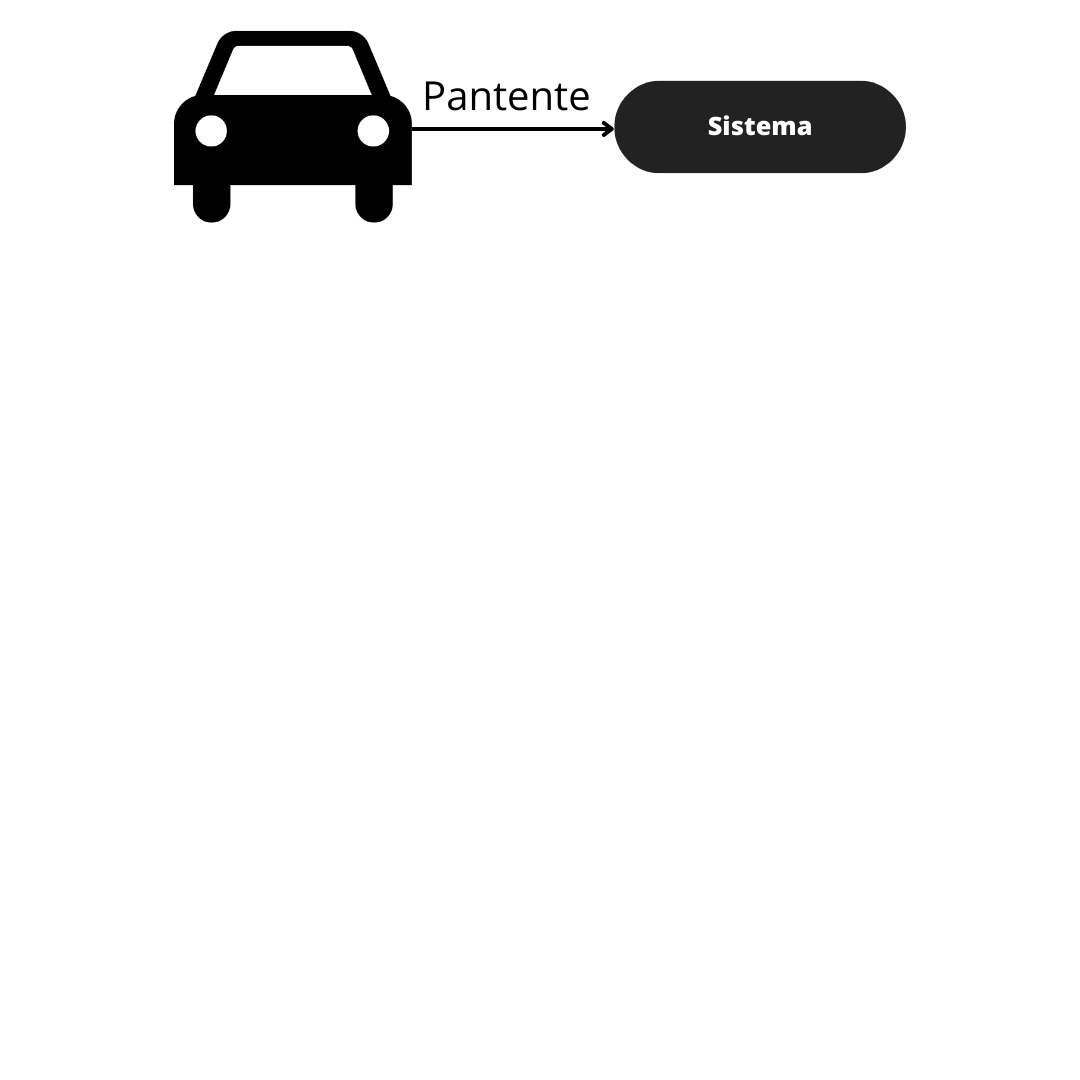
\includegraphics[width=.8\textwidth]{imgs/sistema-base.png}
    \caption[Modelo de caja negra del sistema.]{Idea general del sistema a implementar, en esta versión se toma al bloque de sistema como una caja negra que solo necesita la patente para realizar su tarea.}
    \label{fig:sistema-base}
\end{figure}

De estos requisitos se desprende la forma más general del sistema, que detecta los caracteres del vehículo, permite la identificación del vehículo, y basado en la hora de entrada y salida, calcula el tiempo que estuvo el vehículo, en la Fig. \ref{fig:sistema-base} se observa un modelo de caja negra del sistema.
Existe un gran inconveniente a la hora de obtener el texto de la patente de una imagen y es el tiempo de procesamiento. Es por ello que se utilizará un sensor de distancia para garantizar que existe un objeto.
La versión correspondiente del sistema se puede observar en la Fig. \ref{fig:sistema-completa}.

\begin{figure}[bth]
    \centering
    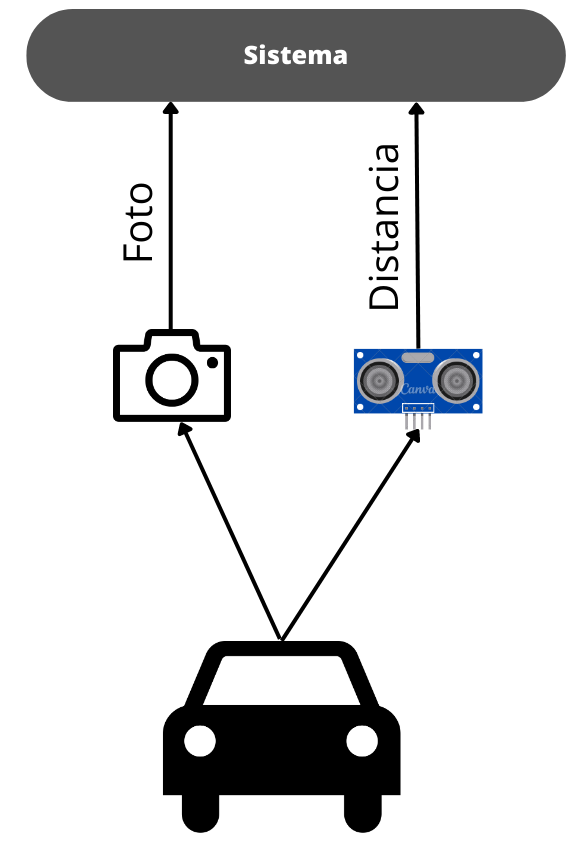
\includegraphics[width=.3\textwidth]{imgs/sistema-con-sensor.png}
    \caption{Sistema con sensor de distancia y cámara.}
    \label{fig:sistema-completa}
\end{figure}

Debido a que los parques de estacionamiento, como los de los supermercados, tienen entradas y salidas diferenciadas, el sistema deberá tener un comportamiento diferente según donde se encuentre.
Es por ello que se implementarán dos algoritmos, uno para manejar las entradas y otro para manejar las salidas.

\section{Algoritmos de entrada y salida}

Una vez establecido como se verá el sistema, se debe definir su comportamiento cuando un vehículo entra o cuando sale.

\subsection{Algoritmo de entrada}

La toma de muestra, es decir, una fotografía, se da cuando el sistema detecta que tiene un objeto a menos de $X$cm. Luego, se procesa la imagen, para obtener la patente en formato de texto.
En caso de encontrar una patente, se almacena la fecha, junto con la patente y la fotografía Fig. \ref{fig:flujo-entrada}.

\begin{figure}[bth]
    \centering
    \begin{subfigure}{.3\textwidth}
        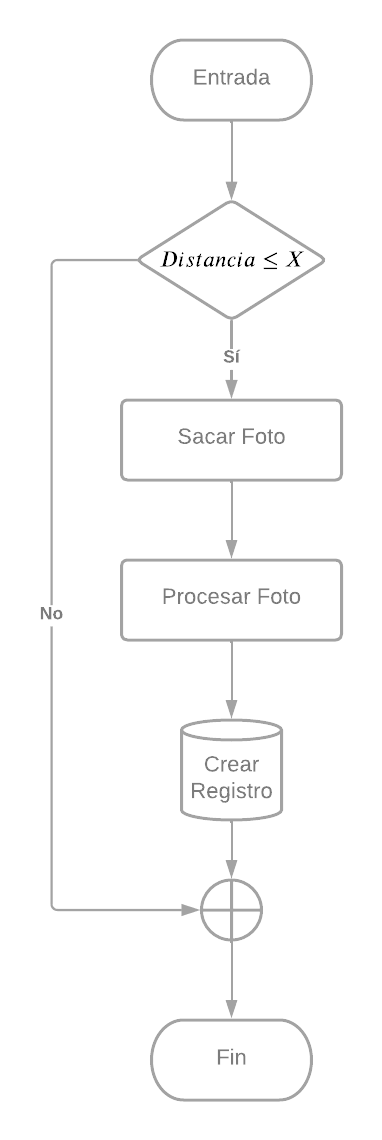
\includegraphics[width=\textwidth]{imgs/flujo-entrada.png}
        \caption{Entrada.}
        \label{fig:flujo-entrada}
    \end{subfigure}
    \begin{subfigure}{.3\textwidth}
        \centering
        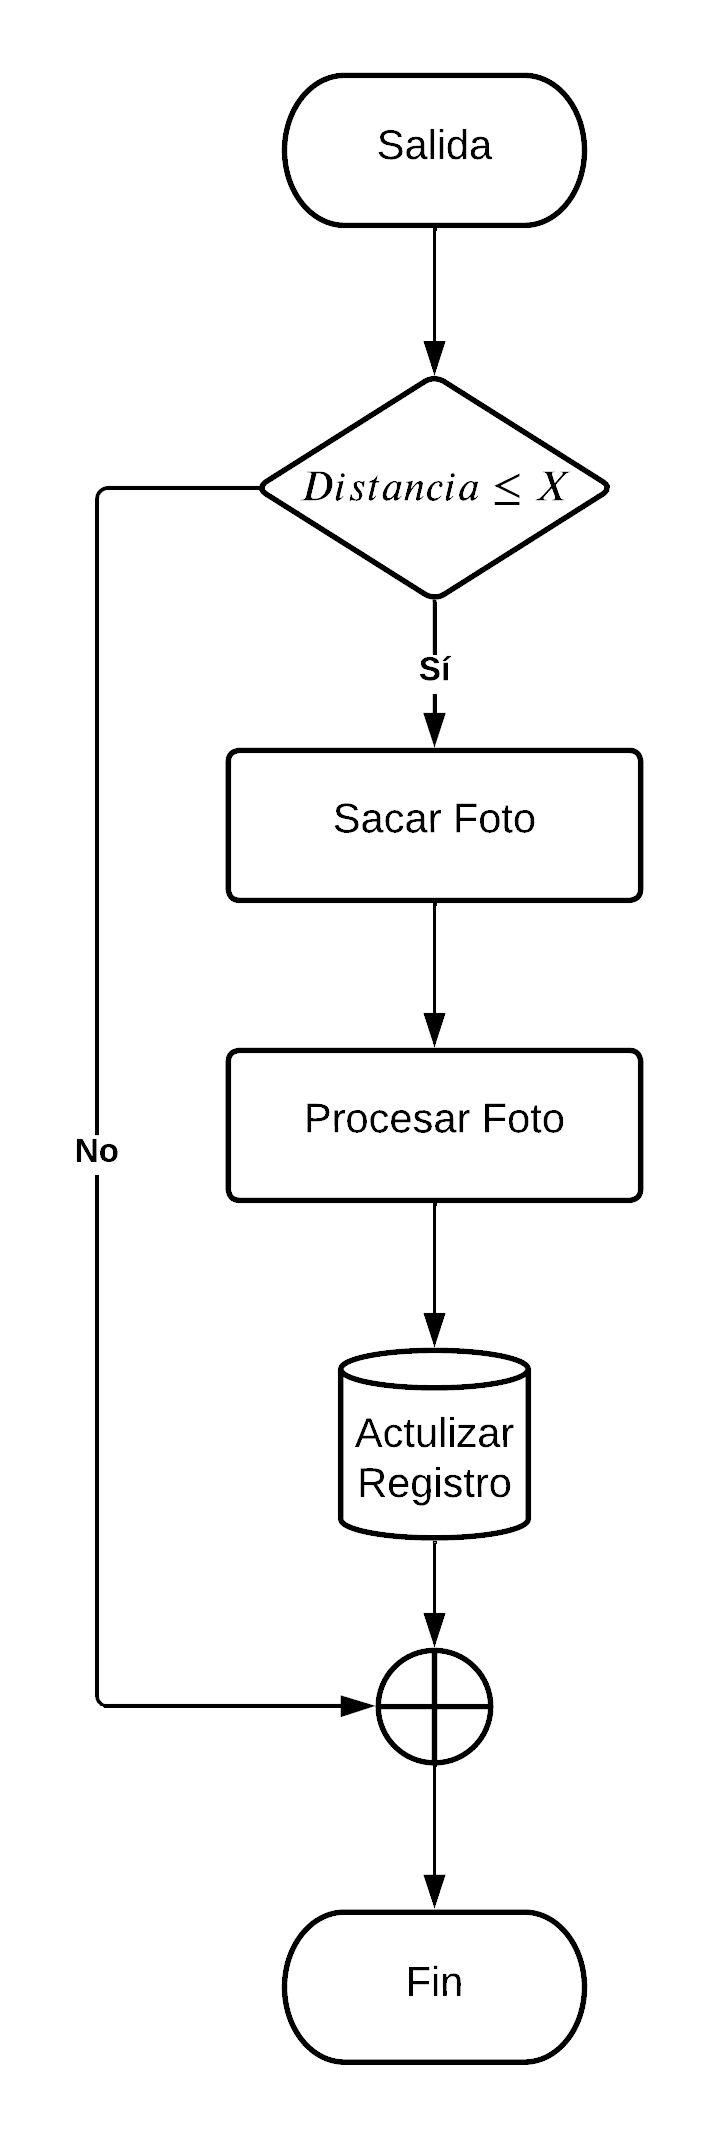
\includegraphics[width=\textwidth]{imgs/flujo-salida.png}
        \caption{Salida.}
        \label{fig:flujo-salida}
    \end{subfigure}
    \caption{Diagramas de flujo para la entrada y la salida de un vehículo del estacionamiento.}
\end{figure}

\subsection{Algoritmo de salida}

El algoritmo de salida es idéntico en la toma de muestra, pero antes de guardar la información de salida (foto y fecha), verifica que exista un registro de entrada correspondiente y se actualiza el mismo Fig. \ref{fig:flujo-salida}.

\subsection{El problema de múltiples establecimientos}

Ambos algoritmos poseen un pequeño inconveniente a la hora de extender el proyecto en más de un recinto. Es por ello que cada barrera se vincula a un lugar, y los registros se buscan y actualizan en función del lugar que tiene asignado cada barrera.

\section{Partes del sistema}

Una vez diseñado y comprendido como está compuesto el sistema a grandes rasgos, es importante entender las partes del mismo y lograr diferenciar que parte del algoritmo se ejecutará en el sistema SL y cuál en el servidor. Para la comunicación del SL con el servidor se optó por utilizar 2 protocolos de comunicación: por un lado HTTP para el envío y actualización de registros de entrada/salida, y MQTT para cambios en la configuración de las barreras.
En la Fig. \ref{fig:sistema-server-barrera} se observa como interactúan los vehículos con la plataforma, la flecha en rojo se utiliza para destacar el envío de datos por MQTT.

\begin{figure}[bth]
    \centering
    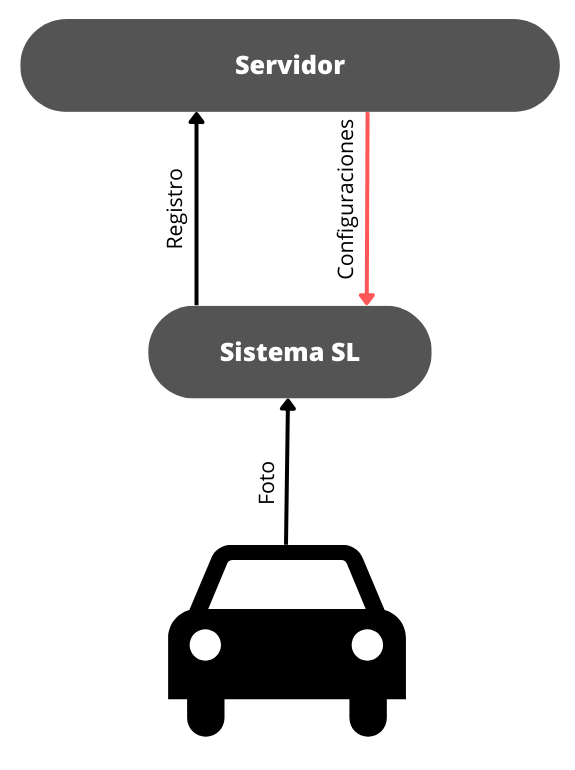
\includegraphics[width=.3\textwidth]{imgs/sistema-server-barrera}
    \caption{Sistema separado en SL y servidor.}
    \label{fig:sistema-server-barrera}
\end{figure}

Esta es la versión que se desarrollará en los capítulos siguientes.

\subsection{Interacción con el cliente}

Debido a que el enfoque del diseño implica un cliente que desea utilizar el sistema se desarrolla una plataforma web para simplificar el manejo de configuración y administración del sistema. En la Fig. \ref{fig:esquema-cliente-servidor-sl} se observa la arquitectura a implementar en el servidor, teniendo en cuenta las interacciones y su manejo entre los sistemas SL y los clientes.
\begin{figure}[bth]
    \centering
    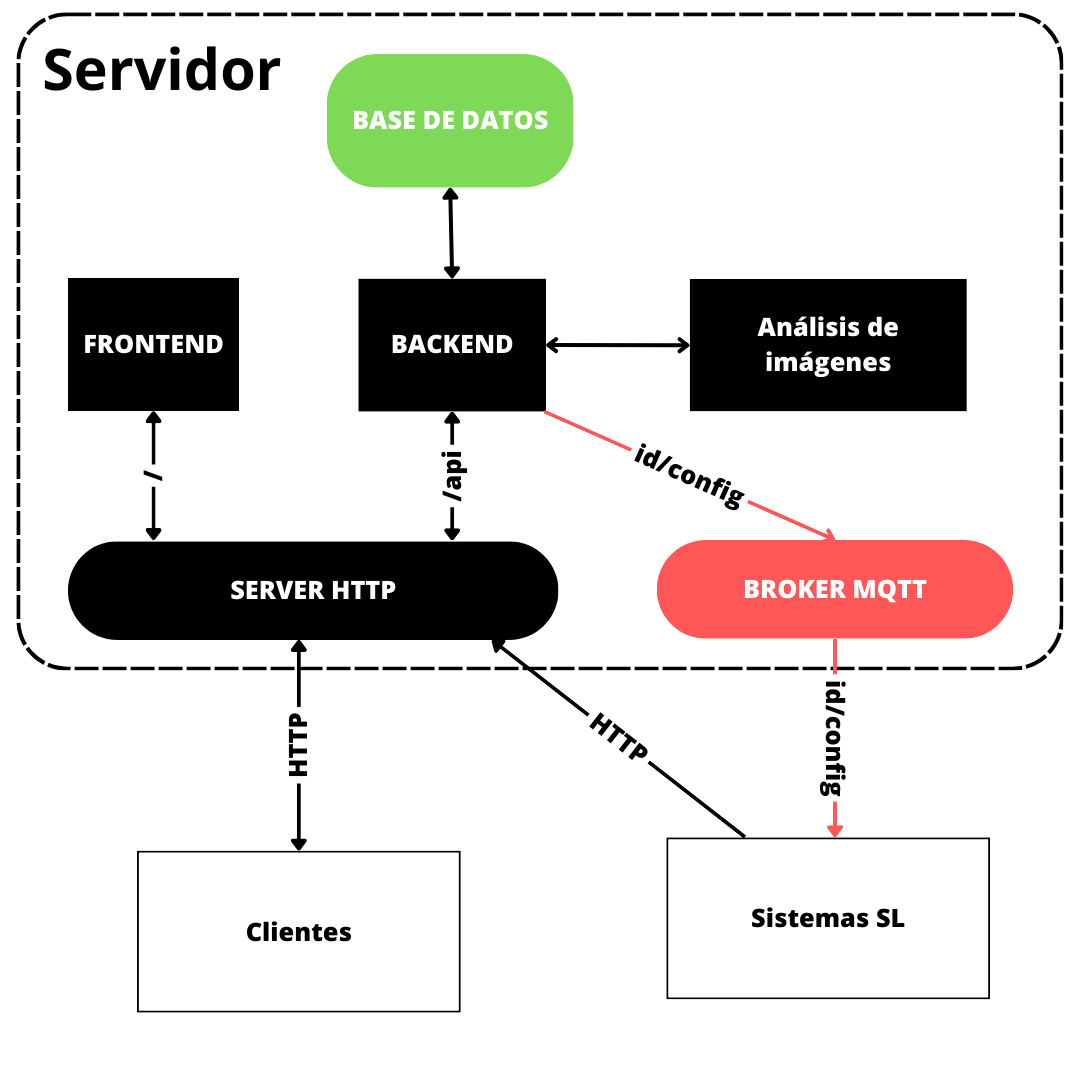
\includegraphics[width=.4\textwidth]{imgs/server-clientes-barreras.png}
    \caption{Esquema de comunicación Cliente-Servidor-SL.}
    \label{fig:esquema-cliente-servidor-sl}
\end{figure}

